\documentclass[11pt, a5paper, parskip=half-, DIV=12]{scrartcl}

\usepackage{../endeavour}
\usepackage{../endeavour_book}

% Hack to allow relative path here
\tikzset{starfield/.pic={
%	\node () at (current page.center) {
\includegraphics[width=\pagewidth, height=\pageheight]{../Images/starfield.png}};
}}

\version{0.1}

\begin{document}
% Colour Cover
\thispagestyle{plain}
\AddToShipoutPictureBG{
\begin{tikzpicture}[remember picture, overlay]
	\node () at (current page.center) {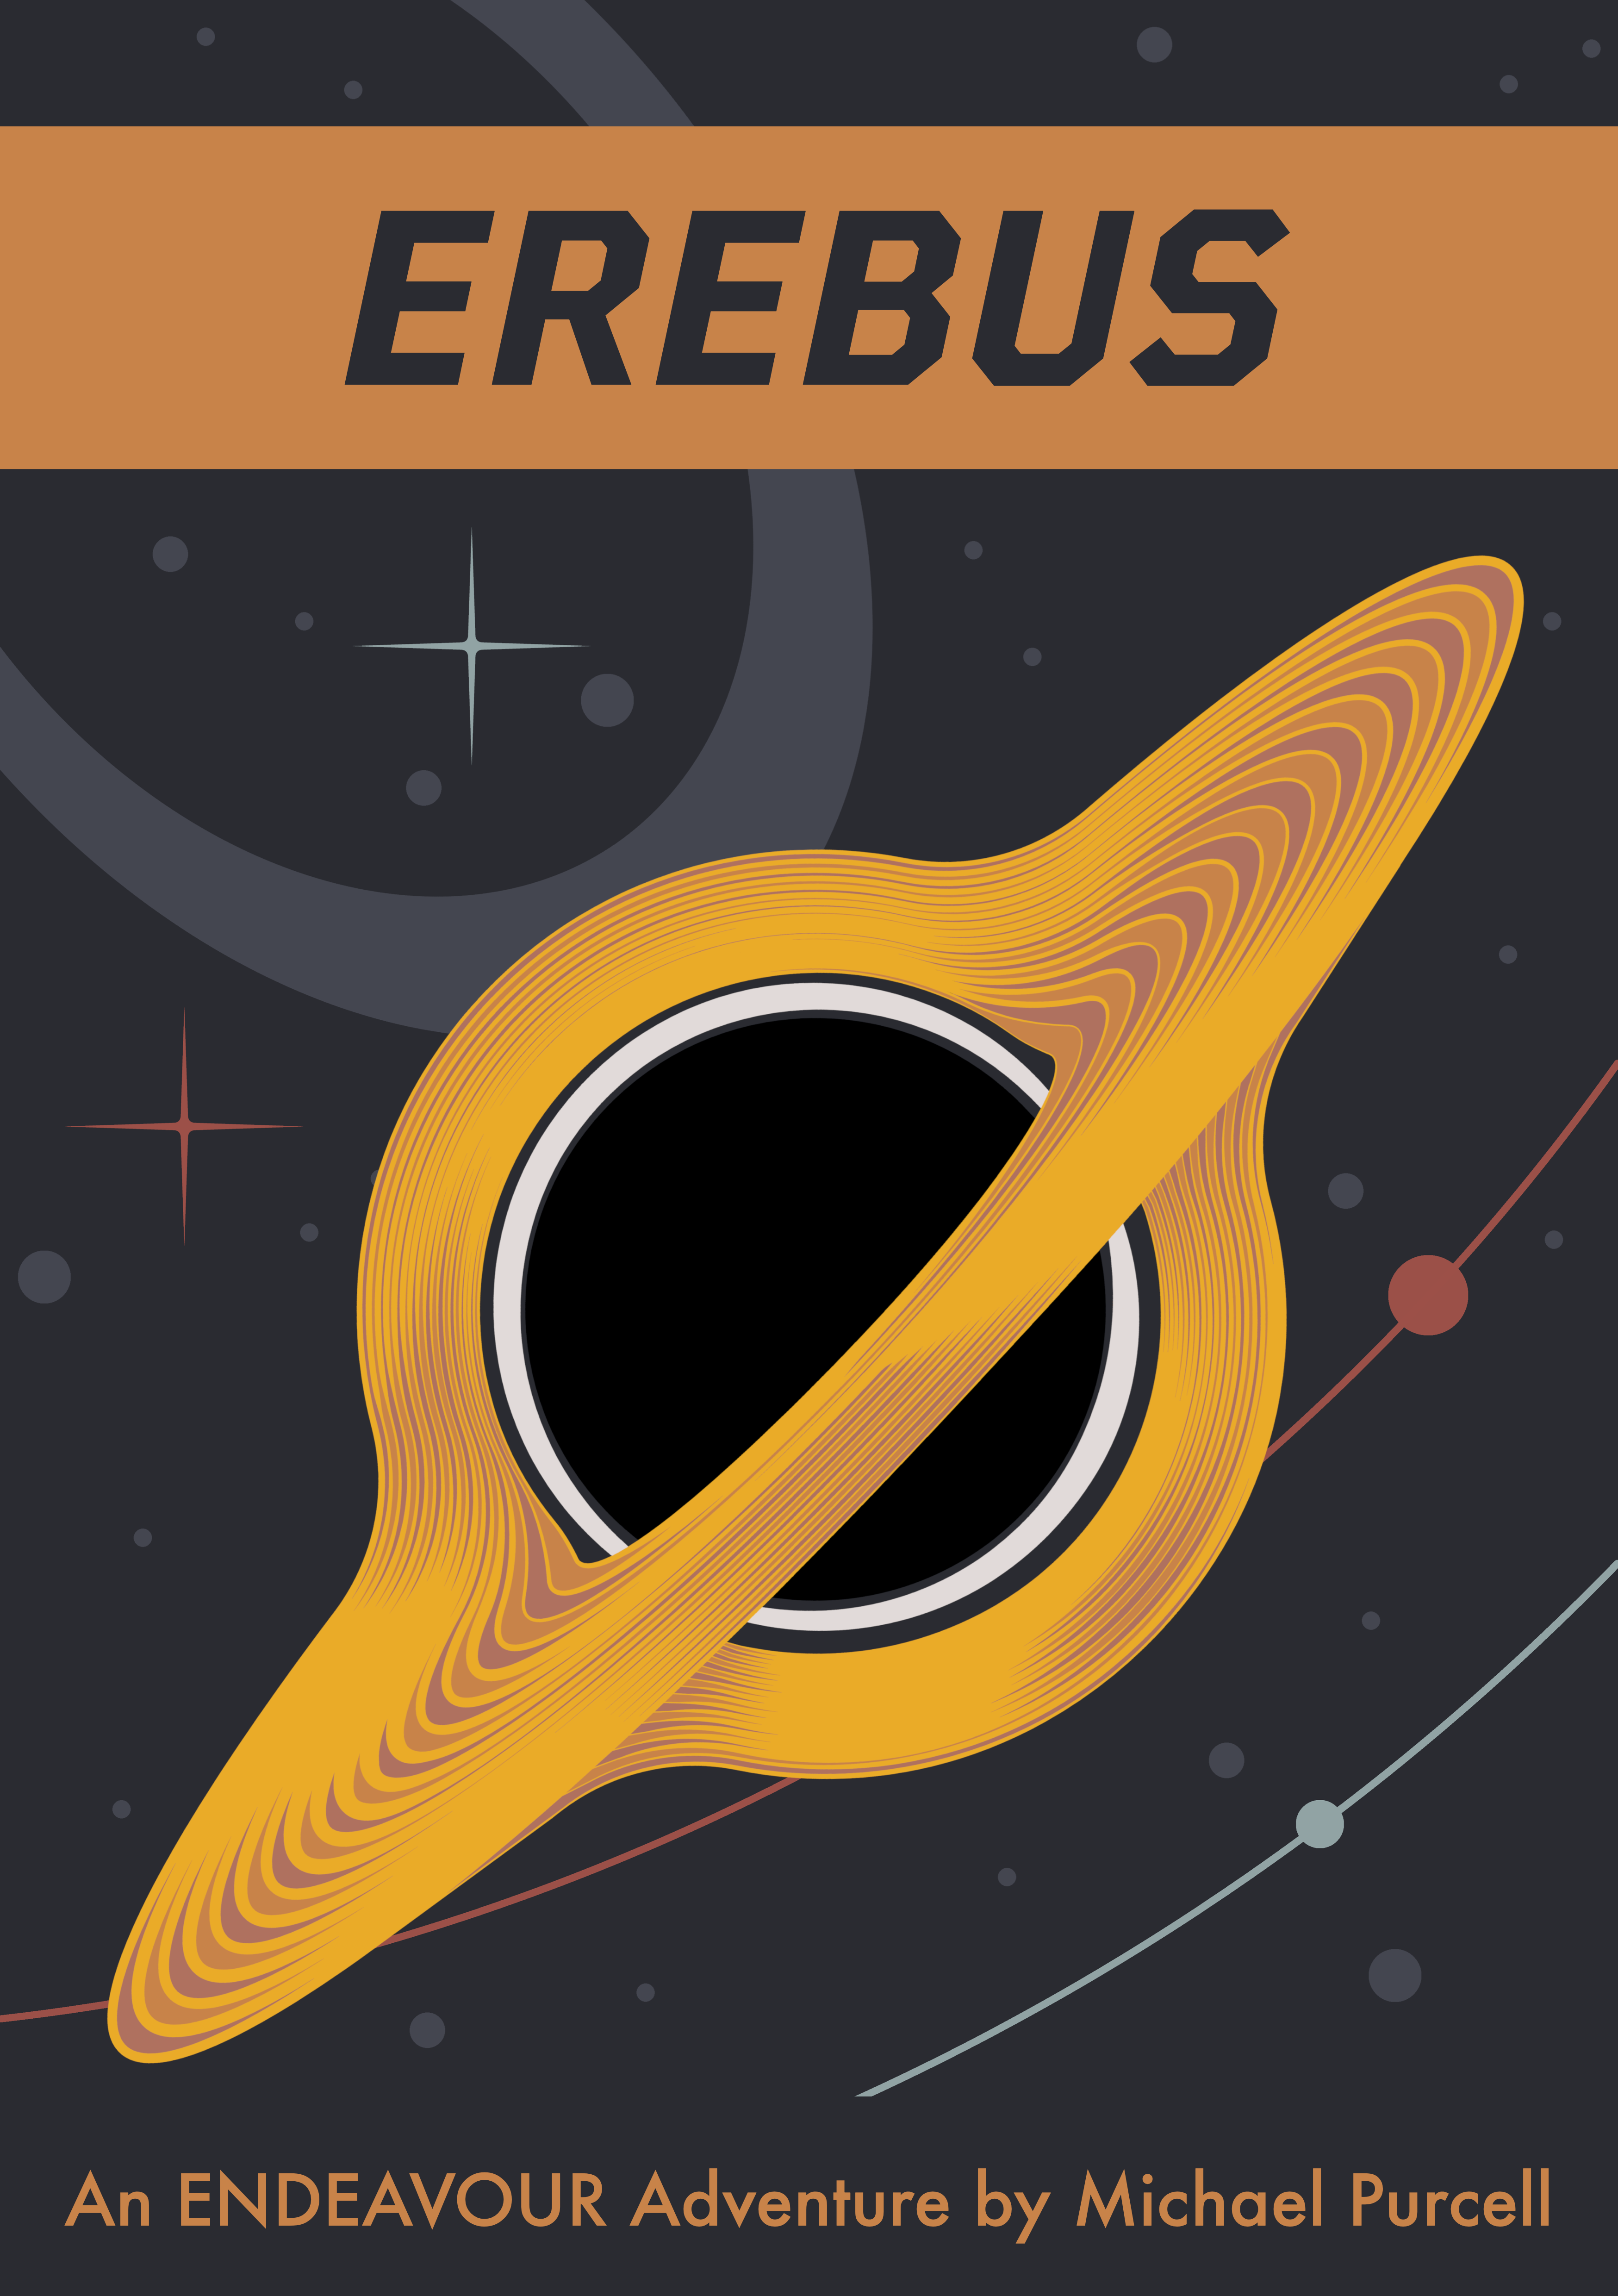
\includegraphics[width=\pagewidth, height=\pageheight]{../Images/erebus_cover.png}};
\end{tikzpicture}
}
{
\colorlet{headfootcolor}{LCARS_ORANGE}
\phantom{a}

\newpage
}

\ClearShipoutPicture
\AddToShipoutPictureBG{
	\begin{tikzpicture}[remember picture, overlay]
	\pic () at (current page.center) {starfield};
		\node[endeavour_box, minimum width=12.6cm, minimum height=18.8 cm] at (current page.center) {};
	\end{tikzpicture}
}

\setcounter{page}{1}
\setmainfont{TeX Gyre Schola}
\normalsize
\raggedright

\section*{Erebus}
\textit{\textbf{Captain's Log:} Several months ago, an ICF survey ship detected unusual emissions coming from Erebus, a black hole far from Interstellar Confederation space. Impossibly, these emissions appeared to be not a natural phenomenon, but rather a transmission sent by an entity known as The Others.}

\textit{Since that time, Erebus has been the subject intense study. We are here to rendezvous with the ICS Discovery, a science ship which has recently been investigating the anomaly.}

\subsection*{Arrival}
\textbf{Zuri Nyota, Captain of the Discovery} welcomes you upon your arrival.  She invites you to come aboard so that she can brief you on recent developments. She reveals that they have decoded the transmission, producing a set of schematics and documentation written in an unknown alien language.

The schematics depict something the crew of the Discovery have taken to calling \textbf{The Device}. They have even managed to reproduce some its components. So far, however, they have not been able to translate the documentation. As such, the purpose of The Device remains shrouded in mystery.

\subsubsection*{Language Barrier}
\begin{itemize}
	\item \textit{Will you try to translate the documentation using only the data that the Discovery has been able to passively collect?} \textbf{Science \& Medicine} vs. \textbf{The Device}. This is a \textit{Grueling} challenge \textendash{} the messages are wholly alien.
	\item \textit{Or will you try to interact with Erebus and establish two-way communication with the messages' sender?} \textbf{Strategy \& Tactics} vs. \textbf{The Others}. This is a \textit{Fraught} challenge \textendash{} the ICF is wary of engaging with anyone who is able to use a black hole as a communications device.
\end{itemize}

\newpage

\subsection*{Trials}

\subsubsection*{Increasing Volatility}
Intermixed with messages from The Others, Erebus begins to emit blasts of high-energy cosmic rays. \textit{Can you maneuver the Endeavour in such a way that you can continue to operate near Erebus without being catastrophically irradiated?} \textbf{Operations \& Engineering} vs. \textbf{Cosmic Rays (2d10)}.

\subsubsection*{Side Effects}
When the science teams begin testing their reconstruction of The Device, ships throughout the area begin experiencing problems with their faster-than-light drives. \textit{Can you determine how the device is interfering with faster-than-light space travel?} \textbf{Science \& Medicine} vs. \textbf{The Device}.

\subsubsection*{Epiphany}
Captain Nyota orders the science teams to suspend their research and lock the files that contain their findings. She seems afraid of something that she has learned about The Device. \textit{Can you convince Captain Nyota to explain what she is afraid of?} \textbf{Leadership \& Negotiation} vs. \textbf{Zuri Nyota}.

\subsection*{Crisis}
The Others want to permanently disrupt faster-than-light travel. To do so, they need you to activate The Device. If you refuse, the Exhaust Universe will be destroyed.

\begin{itemize}
	\item \textit{Will you activate The Device?} \textbf{Threats:} Captain Nyota prevents you from activating The Device. Captain Darcy is arrested and relieved of command. Faster-than-light travel becomes impossible throughout the universe. 
	\item \textit{Or will you refuse to activate The Device?} \\ \textbf{Threats:} The Others use a back door to activate The Device remotely. Captain Darcy resigns his commission. The Exhaust Universe is destroyed.
\end{itemize}

\newpage

\subsection*{Characters}
\begin{description}
	\item[Zuri Nyota (d10):] Captain of the Discovery (d10), Curious (d10), Thorough (d8), Cautious (d8).
	\item[The Others (d10):] Extrauniversal Aliens (d10 \textit{Fraught}), Inscrutable (d10), Earnest (d10), Sophisticated (d10).
	\item[The Device (d12):] Exotic (d12), Self-Sustaining (d12), Mysterious (d10), Powerful (d10 \textit{Dangerous}). 
\end{description}

\subsection*{Places}
\begin{description}
	\item[Erebus:] An intermediate-mass black hole. Surrounded by a luminous accretion disk orbiting at very high speed.
	\item[ICS Discovery:] An ICF science ship. Equipped with advanced sensors, probes, and communication equipment.
	\item[The Exhaust Universe:] A parallel universe in which faster-than-light travel is impossible. Home to many intelligent species and several advanced civilizations.
\end{description}

\subsection*{Mysteries}
\begin{description}
	\item[There are many parallel universes.] \phantom{a} \\ The laws of physics vary from one universe to another. Faster-than-light travel is possible in just two of these universes, The Others' and your own. \textit{Is this peculiarity a result of random chance? Are there other similarities between the two universes? How are they different?}
	\item[Faster-than-light travel damages other universes.] \phantom{a} \\ The Exhaust Universe is on the brink of destruction. Its inhabitants are aware of their predicament but unable to save themselves. \textit{Can you communicate with them? How did The Others learn about the Exhaust Universe? Is it possible to travel between universes?}
\end{description}
\end{document}